\chapter{A reconfigurable continuous-flow fluidic routing fabric using a modular, scalable primitive}
\label{chapter:xposer}
\thispagestyle{myheadings}

% set this to the location of the figures for this chapter. it may
% also want to be ../Figures/2_Body/ or something. make sure that
% it has a trailing directory separator (i.e., '/')!
\graphicspath{{3_xposer/Figures/}}

\section{Introduction}
\label{sec:xposer_intro}
Microfluidic devices, by definition, are required to move liquids from one physical location to another. Given a finite and frequently fixed set of physical channels to route fluids, a primitive design element that allows reconfigurable routing of that fluid from any of  \textit{n} input ports to any \textit{n} output ports will dramatically change the paradigms by which these chips are designed and applied. Furthermore, if these elements are ``regular'' regarding their design, the programming and fabrication of these elements becomes scalable. This paper presents such a design element called a \textit{transposer}. We illustrate the design, fabrication and operation of a single transposer. We then scale this design to create a programmable fabric towards a general-purpose, reconfigurable microfluidic platform analogous to the Field Programmable Gate Array (FPGA) found in digital electronics.

\section{Problem Statement}
\label{sec:xposer_ps}
Engineering frequently involves the exploration of design tradeoffs. Such tradeoffs include time versus quality or performance versus cost \cite{otto1991trade}. A tradeoff frequently encountered in the design of microfluidic systems is specificity versus flexibility. Devices that perform specific tasks often can do these tasks with great precision and quality but users require new devices and/or device architectures for each subsequent task \cite{fidalgo2011}. This lack of re-use increases the cost of experimentation over time, requires re-training for each device, and prevents common platforms for legitimate comparison of results across experiments. Flexible devices on the other hand may not meet stringent performance requirements or the cost of reconfiguring devices may be prohibitively high in terms of time or training \cite{thies2008}. A microfludic device that offers both the performance of a specific solution with the programmability of a flexible solution coupled with low financial as well as time costs would enable entirely new classes of experimentation and design.

Continuous-flow microfluidic chip architectures have yet to fully benefit from the reconfigurable flexibility offered by digital microfluidics \cite{fair2007digital}. Digital microfluidics benefit from extensive research on routing algorithms \cite{curtis2015simulation} that avoid cross-contamination stemming from undesired droplet collisions \cite{cho2008droplet}. These algorithms are predicated on the classification of fluids as discrete droplets, rather than as a continuous-flow. Additionally, digital microfluidic routing algorithms presume that droplets are able to bypass others using a grid of prefabricated paths, combined with the ability to stop the movement of some droplets while continuing to position others \cite{zhao2012droplet}. In contrast, continuous-flow microfluidics must maintain continuous-flow for correct operation of devices such as gradient generators \cite{hung2005continuous}, cell traps \cite{el2006cells}, and batch separators \cite{pamme2007continuous}, thus interrupting flow for the purposes of fluid routing is undesirable. This distinguishes the fluid routing problem from that of a digital microfluidic chip, but it also makes the problem analogous to signal routing in electronic digital design where wires cannot both carry a signal and intersect, which could result in a metastable condition \cite{kleeman1987metastable}.

One approach to the challenge of continuous-flow routing is to examine how reconfigurable computing hardware \cite{todman2005reconfigurable} provides both highly specific, yet programmable, computing elements linked together using a flexible routing fabric \cite{compton2002reconfigurable}. Such an approach retains the specificity of the dedicated resources while allowing those resource relationships (e.g. input and output) to be defined dynamically. Lessons gleaned from the development of modern reconfigurable platforms in the digital electronics domain, namely island-style FPGAs \cite{schmit2005extra}, tell of the need for two major architectural components \cite{kuon2008}:
\begin{enumerate}
	\item Functional primitives that scale regularly, lending to automated design placement
	\item A routing architecture that actuates regularly, lending to automated, dynamic signal routing
\end{enumerate}

These architectural components must then be linked to a control environment using software that scales with the architecture. This requirement prevents chip designers from having to generate artisanal control software for every new chip architecture. As this work demonstrates, the regularity of the primitive and routing structure is what allows for algorithmic scaling in design and control. 

Examples of functional, continuous-flow microfluidic primitives that scale regularly are multiplexors \cite{thorsen2002}, storage elements \cite{thies2008}, culture chambers \cite{fidalgo2011} and mixers \cite{jensen2013}. Chip designs using scalable microfluidic primitives in the absence of a dynamic routing architecture carry similar tradeoffs to those found while designing electronic Application Specific Integrated Circuits (ASICs), whereby the major constraint is that, once implemented, these functional primitives are effectually ``frozen in silicon,'' or in the case of many microfluidic chips: ``frozen in polydimethylsiloxane (PDMS).'' 

\section{Related Work}
\label{sec:xposer_rw}
Microfludics at chip densities belonging to the classes of large scale integration (LSI), i.e., chips with hundreds to thousands of components \cite{thorsen2002}, and very large scale integration (vLSI), i.e., millions of components, have been demonstrated \cite{araci2014}. Electronic Design Automation (EDA) tools for automated design \cite{mcdaniel2013}, layout \cite{huang2014}, and control \cite{thies2008} of these types of chips have also been developed. However, each tool and design paradigm cited above views signal routing as a static problem akin to signal routing in electronic ASIC design, the primary constraint being that continuous-flow channels cannot both carry a signal and intersect on the same fluidic layer without being separated by a valve. EDA tools and chip architectures can overcome this constraint by either incorporating design rules that necessitate the avoidance of channel collisions \cite{huang2014} or dealing with channel collisions individually through the creation of new primitives such as underpasses and vias \cite{huft2013microfluidic}. Additionally, some attempts at channel routing incorporate an element of programmability that necessitates interruption in continuous flow to achieve arbitrary routing \cite{thorsen2002}. These programmable architectures will be be described in further detail in Section \ref{ssec:alts}. What these efforts lack is an ability, integrated into both the chip architecture and control environment, to dynamically route signals to any functional primitive post-fabrication while maintaining continuous-flow and, thus, create a general-purpose fluidic architecture. Only by unlocking this capability can the field of continuous-flow microfluidics expand its design spectrum to include general-purpose platforms among its vast repertoire of application-specific chips thus mirroring the evolution of digital electronics towards experimental pervasiveness. 

This work addresses that need, namely for a scalable, continuous-flow fluidic routing architecture using a network of pre-fabricated channels and integrated software for automated device actuation. A key contribution is the introduction of a ``transposer'' primitive. Transposers allow for a reconfigurable routing fabric. This architecture allows microfluidic chips incorporating high chip densities to better realize the benefits of scaling and come closer to achieving the functional ubiquity of digital electronics.

\section{Primitive Architecture}
\label{sec:primArch}
The theory of operation for a single transposer primitive is shown in Figure \ref{fig:op}. Valves were designed using a monolithic membrane technique previously described \cite{grover2003monolithic}. Briefly, normally closed valving mechanisms are created by introducing discontinuities in a flow channel. These discontinuities are covered by the elastomeric membrane. A corresponding pneumatic cavity is patterned on the control layer \cite{grover2006development}. When a vacuum is introduced into the pneumatic cavity, the elastomer is distended into the cavity, thus allowing flow to proceed in the channel \cite{nguyen2012}. 

A transposer primitive has the ability to selectively swap the contents of two channels, allowing the user to route fluids through the chip dynamically while maintaining continuous-flow. This design requires that one channel ``jump'' over another by traversing between the flow and control layers. One transposer primitive will have two input ports and two output ports. As shown in Figure \ref{fig:modes}, the primitive can take on one of two modes: crossed or straight. In the straight mode, fluids will pass through the primitive unbroken. When the primitive is crossed the contents of both inputs are swapped when viewed from the output ports. 
\begin{figure}[h]
  \begin{minipage}[t]{0.99\linewidth}\centering
    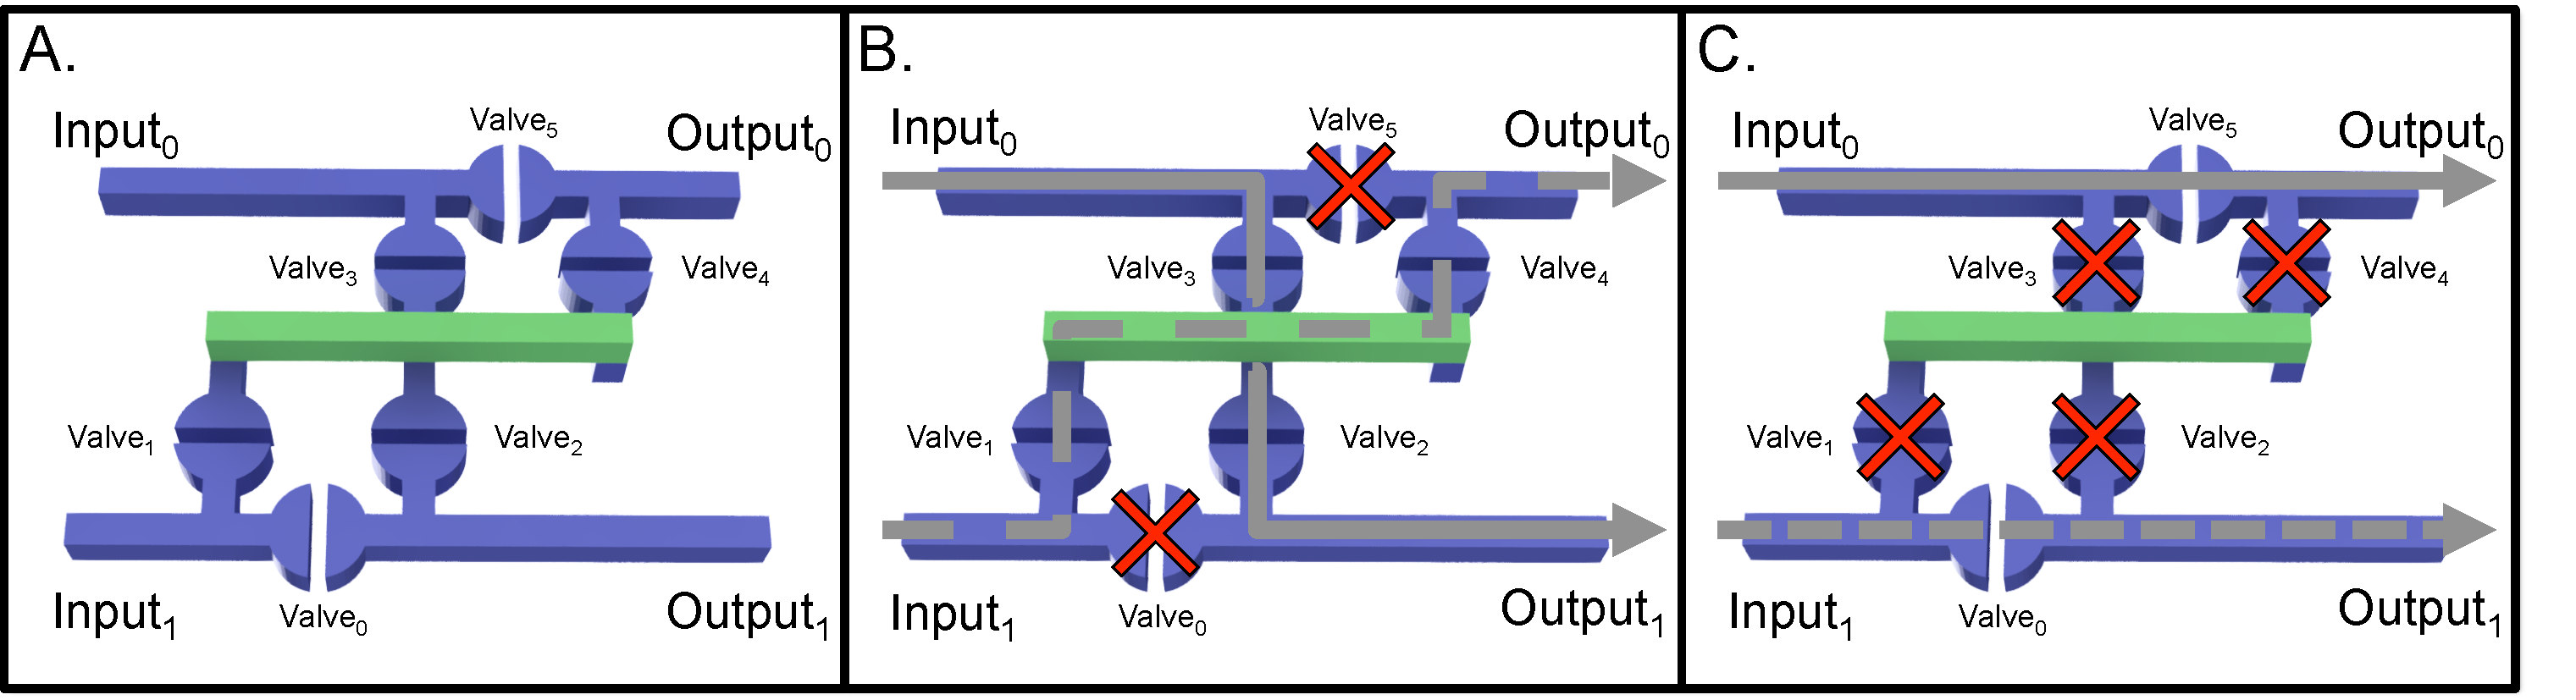
\includegraphics[width=14cm]{fig1.pdf}
    \medskip
  \end{minipage}\hfill
  \caption[Transposer theory of operation]{Theory of operation for a single transposer primitive. A. Normally closed elastomeric membrane valves are realized through discontinuities in flow channels and a corresponding pneumatic cavity on the control layer. The via (green channel) is located on the control layer and is accessed through holes punched in the PDMS membrane. Valves 0 and 5 and valves 1, 2, 3, and 4 are each driven by a single control line, thus one transposer primitive only requires two control lines. B. When valves 0 and 5 are closed and valves 1, 2, 3, and 4 are open the primitive will be in crossed mode in which the fluids will swap channels when viewed from the outputs. C. When valves 1, 2, 3, and 4 are closed and valves 0 and 5 are open the primitive will be in straight mode and fluids will flow straight through the primitive.}
    \label{fig:op}
\end{figure}

Our primitive contains six valves, each of which are not individually addressable. This is to reduce the number of pneumatic inputs required to operate the primitive allowing for greater scalability. Valves 0 and 5 in Figure \ref{fig:op} are controlled by a single control line as are valves 1, 2, 3, and 4; thus the six valves in each primitive only require two control lines for operation.

\subsection{Microfluidic Materials and Assembly}
\label{sec:assembly}
The microfluidic assembly stack for a single transposer primitive is shown in Figure \ref{fig:assembly1}. Channel and valve features were ablated from polycarbonate (PC) (McMaster-Carr, Robbinsville, NJ, USA) using a desktop CNC-mill (Othermill, Othermachine Co., San Francisco, CA, USA). The PDMS membrane was fabricated by mixing a prepolyer (Sylgard 184 Silicone Elastomer Kit, Dow Corning, Midland, MI, USA) with the curing agent at a ratio of 10:1. This mixture was then degassed in a vacuum desiccator. A 250$\mu$m thick PDMS membrane was produced using a method previously described \cite{horner2012}. The via on the control layer, shown in Figure \ref{fig:assembly1}, is accessed through holes punched in the PDMS membrane. Holes were punched by hand using a 1mm biopsy punch (Miltex, York, PA, USA). Flow and control layers were bonded to the PDMS membrane using van der Waals force as described previously \cite{mcdonald2002poly}\cite{duncan2013}. Additional bonding strength was achieved through the use of office binder clips \cite{duncan2015scaling}. The assembled PC-PDMS-PC device stack was then placed in a vacuum desiccator to remove air bubbles created at the material interfaces during assembly.
\begin{figure}[h]
  \begin{minipage}[t]{0.99\linewidth}\centering
    \includegraphics[width=9cm]{fig2.pdf}
    \medskip
  \end{minipage}\hfill
  \caption[Functional, physical, and graphical representations of a transposer]{The functional, physical and graphical representations above demonstrate how the transposer can route fluids straight through the primitive (A.) or swap the inputs when viewed from the output ports (B.). Vertices labeled $v_i$ where $v\in\{S,D,T\}$ correspond to source, decision and terminal nodes, respectively, the formal definitions for which are found in Section \ref{sec:defs}. The $i$ value for source and terminal nodes represent the vertex's level, as there will only be one of each per level, whereas the $i$ value for decision nodes are numbered incrementally by stage, left to right, starting at level 0, stage 1 as described by Algorithm \ref{alg:PopulateVertices}. The addressing node $v_o$ for the single transposer primitive represented above is $D_0$ since it is a decision node that exhibits heteroparity of coordinates (i.e., $p_l+p_s$ is an odd number).}
	\label{fig:modes}
\end{figure}

\begin{figure}[h]
  \begin{minipage}[t]{0.99\linewidth}\centering
    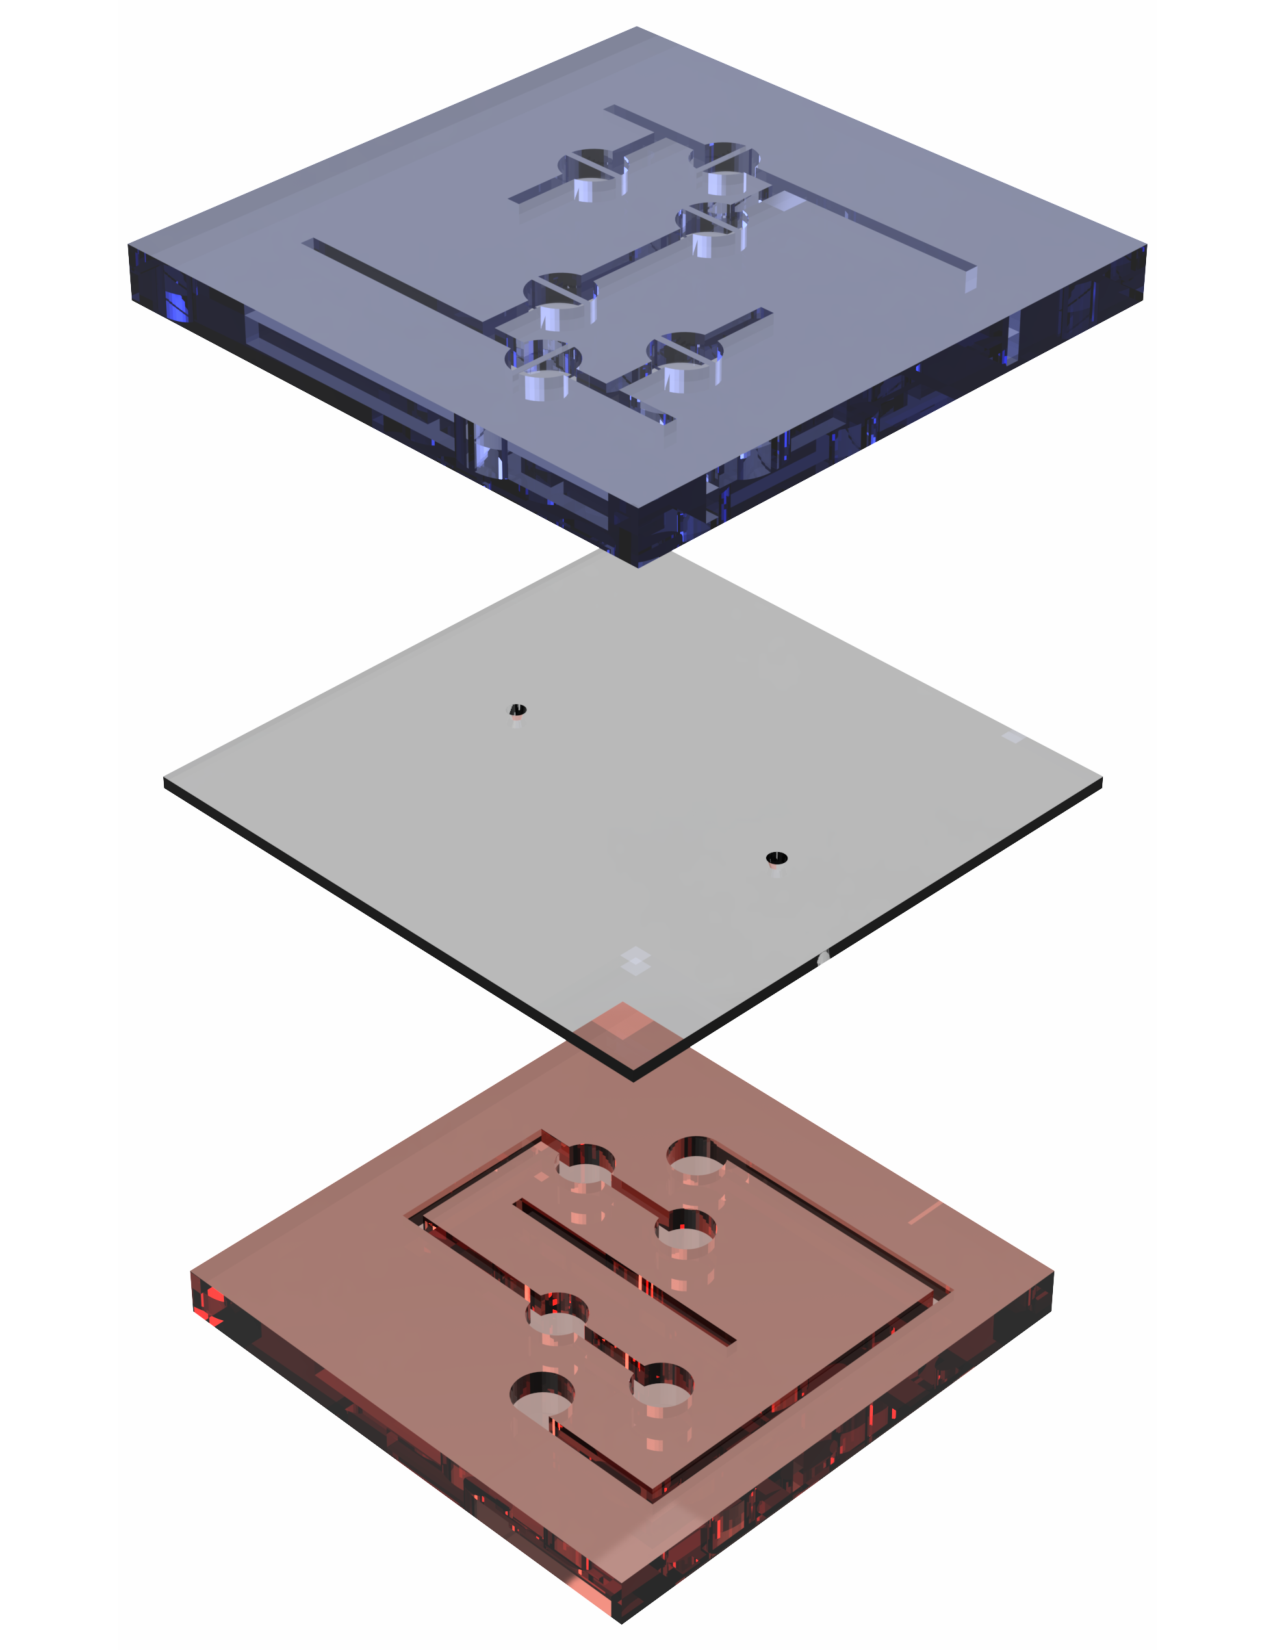
\includegraphics[width=9cm]{fig3.pdf}
    \medskip
  \end{minipage}\hfill
  \caption[Microfluidic assembly stack for a transposer]{Microfluidic assembly stack. Channel and valve geometries in flow (blue) and control (red) layers were ablated from polycarbonate. The via on the control layer is accessed from the flow layer by through-holes punched in the PDMS membrane that separates the two polycarbonate layers.}
	\label{fig:assembly1}
\end{figure}

\subsection{Routing Fabric Definitions}
\label{sec:defs}
In order to generate an algorithm that automatically routes fluids through the routing fabric to their desired destinations we begin by representing the transposer-based routing fabric as a \textbf{directed acyclic graph} (DAG). A \textbf{graph} $G=(V,E)$ is a data structure consisting of a set of \textbf{vertices} $V$ and a set of \textbf{edges} $E$ connecting these vertices \cite{vaidyanathan2015}. A \textbf{directed graph} is a subset of graphs in which all edges are ordered pairs of elements $(v_i, v_t) \in V$. An edge $e_{it}$ begins with an \textbf{initial vertex} $v_i$ and ends in a \textbf{terminal vertex} $v_t$. A \textbf{path} from $v_0$ to $v_n$ is an ordered set of edges $(v_0, v_1),(v_1,v_2),(v_2,v_3),\cdots ,(v_{n-1},v_n)$, such that the terminal vertex of each edge is the same as the initial vertex of the next edge in the path. In an \textbf{acyclic graph}, there exists no path that starts with a vertex $v_i$ and ends with the same vertex $v_i$.

An \textbf{unrouted} graph will contain all possible edges in the routing fabric, however since each individual primitive has only two modes (crossed and straight) not all combinations of edges are possible. Figure \ref{fig:algProgression}C shows an unrouted graph for a three-input fabric of transposer primitives. A \textbf{routed} graph contains only the edges used to route source nodes to the terminal nodes set by a user. Figure \ref{fig:modes} shows examples of routed graphs for a single transposer in each primitive mode, straight and crossed. A vertex is a \textbf{decision node} when it is a terminal vertex for at least one edge and an initial vertex for exactly two other edges in the unrouted graph and exactly one other edge in a routed graph. A vertex is a \textbf{source node} when it is not a terminal vertex for any edge in the graph. A vertex is a \textbf{terminal node} when it is not an initial vertex for any edge in the graph.

Each source node occupies a horizontal \textbf{level} in the graph. At a decision node, the next edge in the graph may either stay on the same level or traverse a level. The direction of the traversal (either increment a level or decrement a level) depends on the position of the vertex, as described in Section \ref{sec:unrouted}. For example, the decision node $D_0$ in Figure \ref{fig:modes} may either traverse from level 0 to level 1, thus incrementing a level, or stay on level 0, whereas the decision node $D_1$ may only traverse from level 1 to level 0, thus decrementing a level, or stay on level 1. Each vertex occupies a vertical \textbf{stage} in the graph. All edges in the graph traverse stages. For each vertex $v\in V$, $\exists$ a set of points $p=p_l,p_s$ that represent the vertex's coordinates expressed in terms of level, $l$, and stage, $s$.

Microfluidic elements are mapped onto a graph framework in order to translate the results of a graph traversal into proper fluid flow on a physical device. \textbf{Flow ports} are placed at all source (input) and terminal (output) nodes. One \textbf{control port} must be placed on each channel of equipotential in the control layer shown in Figure \ref{fig:assembly1}, with the exception of the via. Based on this requirement, each primitive requires two control ports. A \textbf {transposer primitive} $x_o$ is addressed by a single decision node $v_o \in V$. $v_o$ is said to have heteroparity of coordinates (i.e., $p_l+p_s$ is an odd number). A list of transposer primitives $X$ maintains the locations of each individual primitive $x_o$ addressed by $p_{v_{o}}$.

\section{Theory of operation}
\subsection{Scalable Routing Fabric}
A single transposer primitive can route fluids from two different input channels to two different output channels. A routing fabric, by definition, is composed of multiple transposer primitives and can be built to allow for fluid routing of $n$-input channels. The architecture on which this fabric is built is a mason layout, which can be defined as an array of primitives with either homoparity or heteroparity of coordinates; our fabric arranges primitives based on heteroparity of coordinates to account for source nodes at stage 0. The scaling of such an architecture is demonstrated in Figure \ref{fig:fabric}. The number of primitives scales according to the number of inputs, $n$, as defined by the recursively defined function in Equation \ref{eqn:fabric}. Since a single transposer primitive can route two inputs, the number of primitives required to route an $n$ less than two would be zero.

\begin{equation}
  \label{eqn:fabric}
  f(n)= \begin{cases} 0, & \mbox{if } n\mbox{ is } <2 \\ f(n-1)+n-1, & \mbox{if } n\mbox{ is } \geq 2 \end{cases}
\end{equation}

Thus, for $n\geq 2, f(n) = \sum_{i=1}^{n-1} i = n \cdot (n-1) / 2 \in \Theta(n^2).$ 

    \begin{figure}[h]
     \begin{minipage}[t]{0.99\linewidth}\centering
      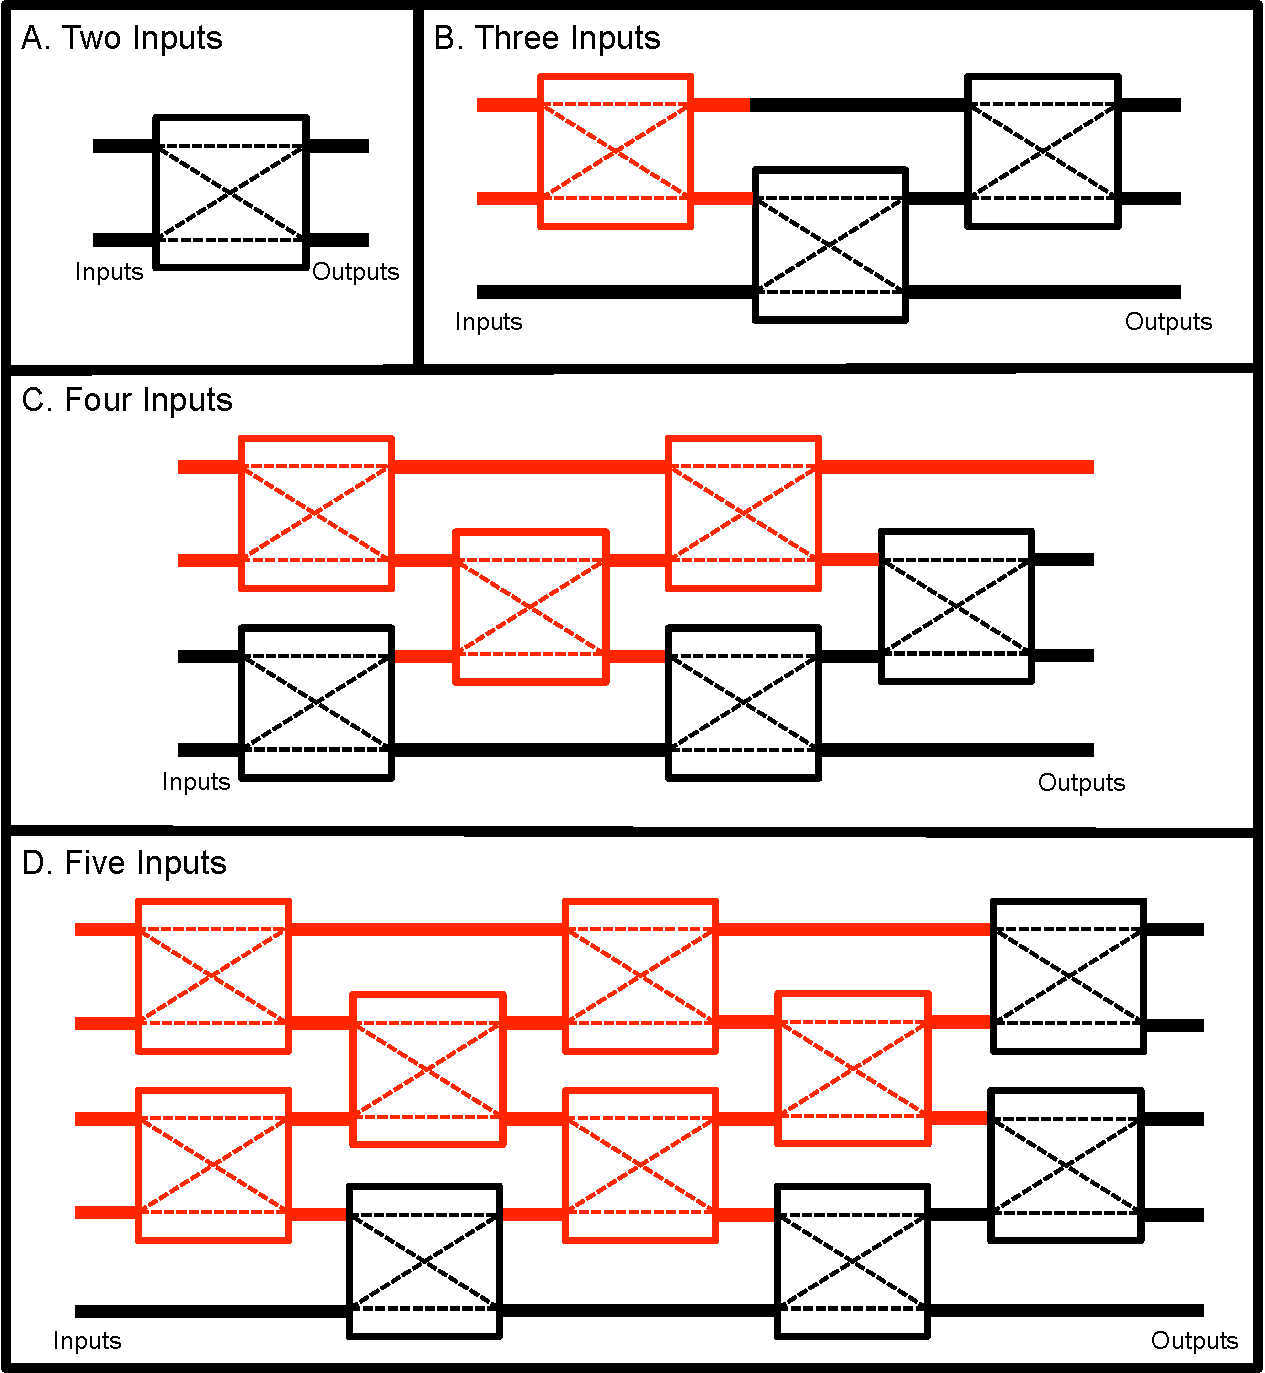
\includegraphics[width=9cm]{fig4.pdf}
      \medskip
     \end{minipage}\hfill
     \caption[Examples of a populated routing fabric]{Examples of a populated routing fabric. A. shows a single primitive, represented as a box, which is able to route two fluidic inputs to two fluidic outputs. This primitive (highlighted in red in B.) can be tiled with two other primitives, thus enabling the ability to route three fluidic inputs. The addition of three primitives (C.) to the three-input architecture (red) results in a four-input fabric. D. shows the natural continuation of the tiling process by adding four additional primitives to the four-input fabric (red) in order to create a five-input fabric. The number of transposer primitives required $f(n)$ for A--D is 1, 3, 6 and 10, respectively, as dictated by Equation \ref{eqn:fabric}.}
	    \label{fig:fabric}
    \end{figure}



\subsection{Optimality of the number of transposers}

Below, we show that a quadratic number of transposers is necessary and sufficient for routing any permutation of $n$ inputs to $n$ outputs.

\subsubsection{Necessity}

Routing an arbitrary permutation of $n$ inputs requires reordering the input fluids using transposers, in such a way that they arrive at their intended output destinations. We observe that each transposer is capable of reordering exactly two channel positions. Consider the scenario where inputs $i$ must be routed to output $n-i+1$. Here, input $i$ must require $|n-i+1-i| \in \Theta(n)$ transpositions, and therefore $\Theta(n)$ transposers. Thus, to route all $n$ input channels in this case, the problem scales on the order of $\Theta(n^2)$ transposers. It is important to note that this is a claim regarding the routing problem's complexity; the actual number of transposers required is described in Equation \ref{eqn:fabric}.

\subsubsection{Sufficiency}

Routing is accomplished by correctly routing an initial input to its destination, and then recursing. In this fashion, all inputs can be routed based on the necessary condition outlined above. The definition of correct routing is described in Section \ref{ssec:correct}.

\subsection{Planar and non planar fabrics}
Consider a graph with a vertex for each transposer and an arc from vertex $u$ to $v$ if fluid can flow directly out of the transposer corresponding to vertex $u$ into that corresponding to vertex $v$, without flowing through any  transposers along the way. It is easy to observe that this graph is planar for any $n$-input fabric. The ``intersection'' of flows occurs within a transposer. For planar fabrics, the above argument shows that the fabric design described is optimal in the number of transposers. 

\subsection{Comparison with alternative primitives}
\label{ssec:alts}
Similar programmable routing could be achieved using existing primitives. For example, a one-of-$n$ input could be routed to any of $n$ outputs using a multiplexer-demultiplexer pair with $\Theta(\lg n)$ control lines \cite{thorsen2002}. Additionally, this design would not allow for continuous-flow across all $n$ input channels, as multiplexors and demultiplexers are one-of-$n$ and $n$-of-one devices, respectively. Flow in channels not selected would, therefore, be stopped. A naive way to obtain an $n$-input $n$-output routing fabric from this would be to use $n$ mux-demux pairs resulting in $\Theta(n \lg n)$ control lines. Such a design, however, would be complex and non planar. Conversely, sub quadratic non planar fabric designs may exist, but we do not explore them here.

\subsection{Analysis of control requirements}
Since each transposer primitive requires two control lines, the number of control lines also scales on the order of $\Theta(n^2)$ with the actual number of control lines required equaling $n(n-1)$. Ballooning control requirements is a fundamental weakness of microfluidic LSI. This weakness has been largely mitigated through the use of microfluidic multiplexors \cite{thorsen2002}. The microfluidic multiplexor creates an infrastructure in which $m$ valves are controlled using $2 log_2(m)$ control lines. Thus, if a microfluidic multiplexor is integrated into to the routing fabric's control framework using latched or unlatched multiplexed addressing, as previously described \cite{melin2007}, the number of control channels would scale at $2log_2[n(n-1)]$ and as such 32 fluids could be routed with 20 control lines and the number of fluids able to be routed would increase exponentially with each additional control line (ex. 50 control lines will arbitrarily route 5,798 fluids). 
\section{Routing Algorithm}
\label{ssec:alg}
There are two main steps in our algorithm for routing within a transposer fabric:
\begin{enumerate}
	\item Generate an unrouted graph based on the number of inputs to be routed $n$
	\item Delete unnecessary edges based on desired fluid destinations to form a routed graph 
\end{enumerate}
Locations on a graph are described in terms of stages and levels. A graph for $n>2$ will have $n$ levels and $n+2$ stages, the additional two stages are a result of source and terminal nodes. Coordinates are zero-indexed. 
    \subsection{Generate Unrouted Graph}
    \label{sec:unrouted}
    Generating an unrouted graph for $n>2$ requires three primary steps:
	\begin{enumerate}
			\item Populate vertices according to rules set forth in Algorithm \ref{alg:PopulateVertices}.
			\item Assign vertices to individual transposers according to Algorithm \ref{alg:PlaceXposers}.
			\item Create edges to form an unrouted graph.
		\end{enumerate}

    \subsubsection{Populate Vertices}
    The first step in generating an unrouted graph for $n>2$ is to populate the vertices based on the number of inputs, $n$. Vertices are placed based on a set of rules. Source nodes are placed on stage 0 of each level, while terminal nodes are placed on stage $n+1$, remembering that coordinates are zero-indexed. There are two main edge cases when placing decision nodes, Level 0 and Level ($n-1$). Placing nodes on all other levels is regular as demonstrated by Algorithm \ref{alg:PopulateVertices}.

\begin{figure}
\begin{algorithm}[H]
\DontPrintSemicolon
\SetKwData{level}{level}\SetKwData{stage}{stage}\SetKwData{stages}{stages}
\SetKwFunction{AppendToV}{AppendToV}
\KwData{Number of inputs to be routed $n$}
\KwResult{A list of vertices $V$}
\Begin{
$levels \leftarrow n-1$\;
$stages \leftarrow n+1$\;
$count \leftarrow 0$\;
$V \longleftarrow \emptyset$\;
  %\tcc{Populate source and terminal nodes}
  \For{Each \level}{
	  $S_{level} \longleftarrow p=level,0$\;
	  $T_{level} \longleftarrow p=level,n$\;
	  $\AppendToV(S_{level})$\;
	  $\AppendToV(T_{level})$\;
  }
\tcc{Populate decision nodes}
  \For{Each \level}{
	  \For{\stages 1 \textbf{through} n}{
      \If{\level$= 0$ \textbf{and} \stage is odd}{
	$D_{count} \longleftarrow p=\level,\stage$\;
	$\AppendToV(D_{count})$\;
      }
      \ElseIf{\level$=n-1$}{
	      \If{$n$ is odd \textbf{and} \stage is even}{
		$D_{count} \longleftarrow p=\level,\stage$\;
		$\AppendToV(D_{count})$\;
	      }
	      \ElseIf{$n$ is even \textbf{and} \stage is odd}{
	 	$D_{count} \longleftarrow p=\level,\stage$\;
		$\AppendToV(D_{count})$\;
	      }
      }
      \ElseIf{\level$\neq 0$ \textbf{or} \level$\neq n-1$}{
	$D_{count} \longleftarrow p=\level,\stage$\;
	$\AppendToV(D_{count})$\;
      }
      Increment $count$\;
    }
  }
}
\caption{Populate Vertices. Creates vertices and assigns coordinates $p$ and type characteristics $v\in\{S,D,T\}$ to each created vertex.\label{alg:PopulateVertices}}
\end{algorithm}
\end{figure}

\subsubsection{Place Transposers}
  Individual transposers $x_o$ are addressed by a single decision node $v_o$ that exhibits heteroparity of coordinates (i.e., $p_{l_{v_o}}+p_{s_{v_o}}$ is odd). Since $v_o$ can only be of type $D$, for decision node, this excludes all vertices in stage 0 (source nodes) and stage $n+1$ (terminal nodes). Once $v_o$ is identified for all transposers in a graph, it is then possible to correctly create edges to form an unrouted graph. Algorithm \ref{alg:PlaceXposers} takes the list of vertices $V$ generated by Algorithm \ref{alg:PopulateVertices} and searches for decision nodes with heteroparity. The algorithm then creates a new transposer primitive $x_o$, assigns it an address $p_{v_{o}}$ and adds the individual transposer to the set of transposers $X$. 

\begin{figure}
\begin{algorithm}[H]
\DontPrintSemicolon
\SetKwFunction{AppendToX}{AppendToX}
\KwData{A list of vertices $V$}
\KwResult{A list of transposer objects $X$}
\Begin{
$X \longleftarrow \emptyset$\;
\For{$v \in V$ where $p_{s_v}\neq 0$ \textbf{or} $p_{s_v} \neq n+1$}{
	  \If{$p_{l_v}+p_{s_v}$ is odd}{
      $x_o \longleftarrow v$\;
      $\AppendToX(x_o)$
    }
  }
}
\caption{Place Transposers. Finds all decision nodes with heteroparity of coordinates, creates a new transposer object $x_o$ in that location and adds the new transposer to the set of transposers $X$ \label{alg:PlaceXposers}}
\end{algorithm}
\end{figure}

\begin{figure}[h]
     \begin{minipage}[t]{0.99\linewidth}\centering
      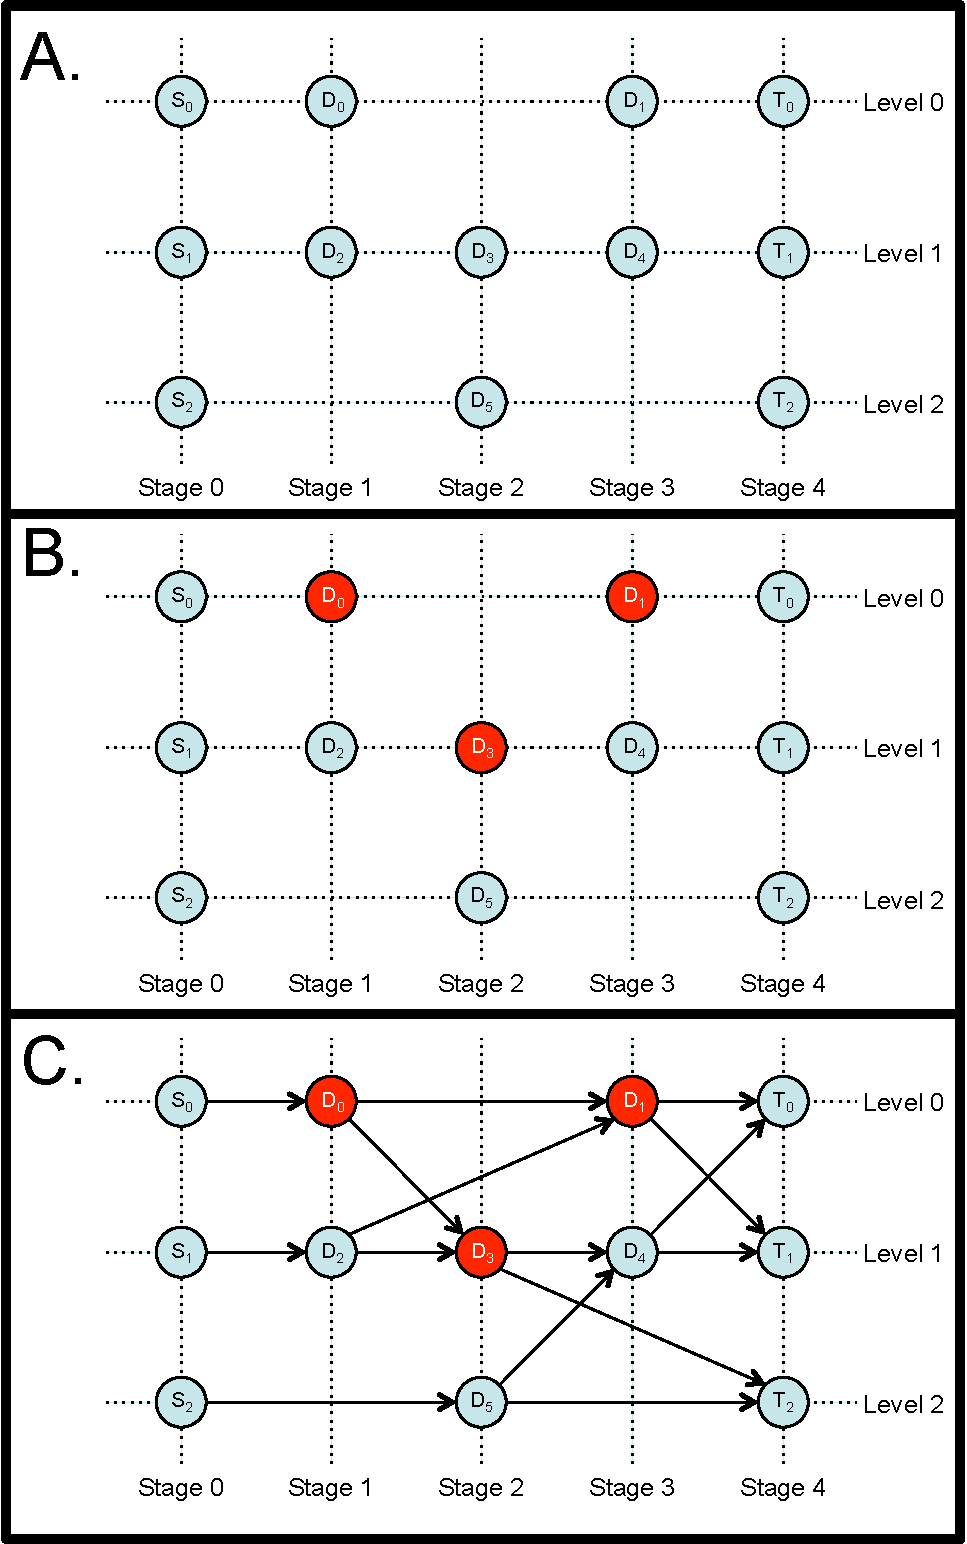
\includegraphics[width=6cm]{fig5.pdf}
      \medskip
     \end{minipage}\hfill
     \caption[Transposer routing algorithmic progression]{Algorithmic progression for generating an unrouted graph for a three-input ($n=3$) routing fabric. A. shows the outcome of Algorithm \ref{alg:PopulateVertices}, where vertices $v_i$ have coordinates $p$ and types $v\in\{S,D,T\}$ corresponding to source, decision and terminal nodes, respectively. B. shows in red the locations of the three transposer primitives as dictated by Algorithm \ref{alg:PlaceXposers}. The number of primitives is governed by Equation \ref{eqn:fabric} and the primitives are defined by their addressable node $v_o$. The graph in C. is the complete unrouted graph as dictated by Algorithm \ref{alg:GenerateGraph}.}
	\label{fig:algProgression}
\end{figure}

\begin{figure}[h]
     \begin{minipage}[t]{0.99\linewidth}\centering
      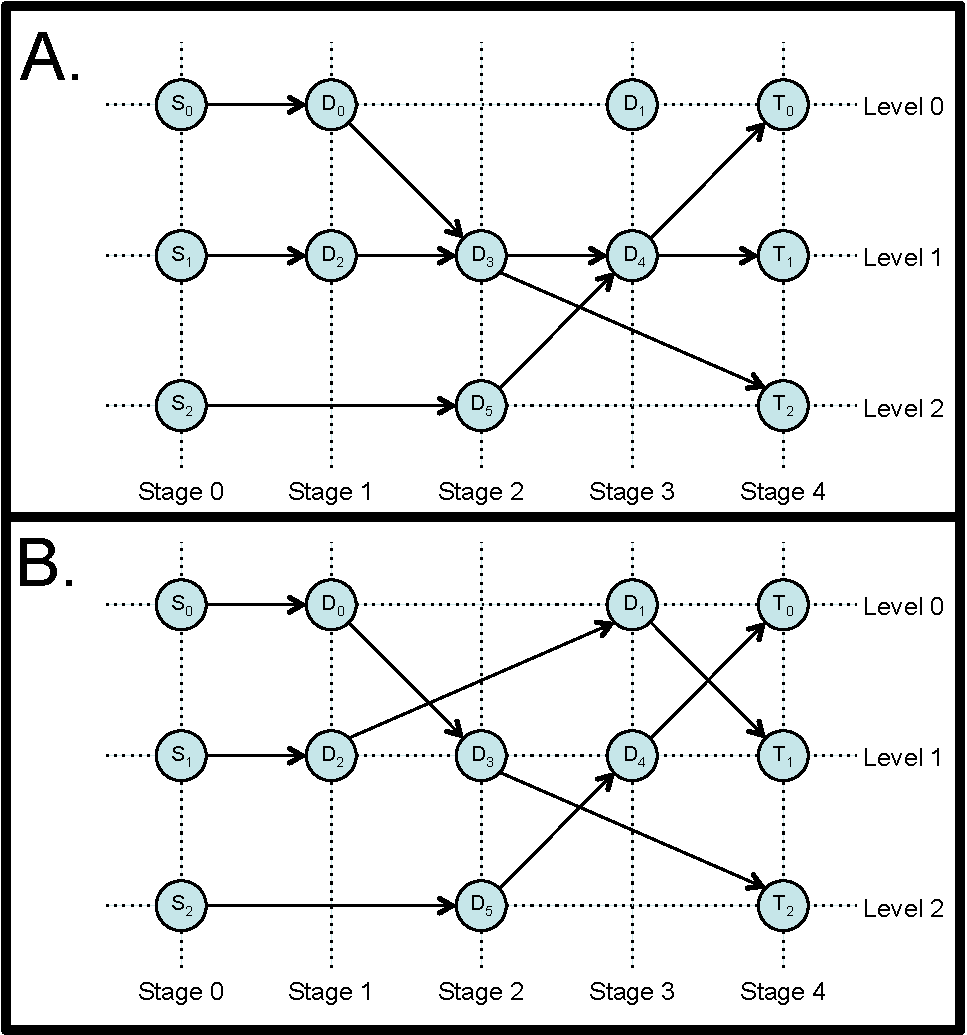
\includegraphics[width=9cm]{fig6.pdf}
      \medskip
     \end{minipage}\hfill
     \caption[Graphical representations of an illegally routed versus a correctly routed graph]{Graphical representations of illegally routed (A.) and correctly routed (B.) graphs. Each graph routes inputs from $S_0$ to $T_2$, $S_1$ to $T_1$ and $S_2$ to $T_0$. The graph in A. is illegal because vertices $D_3$  and $D_4$ appear in more than one path.}
    \label{fig:legalese}
\end{figure}


\subsubsection{Generate Unrouted Graph}
This step links the vertices in list $V$ with edges and, upon completion, results in an unrouted graph that represents a fabric of transposers for $n$ inputs. Algorithm \ref{alg:PlaceXposers} ensures that for each transposer $x\in X$, $\exists$ a decision node $v_o\in V$, and $v_o$ has the characteristic of heteroparity of coordinates; these characteristics make it possible to correctly link all vertices with edges that will form an unrouted graph representing a fabric of transposer primitives. 
    
The first edge will connect $v_o$ to the next vertex on the same level as $v_o$, i.e., $p_{l_{v_o}}$; therefore, the initial vertex for this edge will be $v_o$ and the terminal vertex will be the infimum of the set of vertices on $p_{l_{v_o}}$ with a stage number greater than $p_{s_{v_o}}$. The second edge will be the same as the first except that the terminal vertex will be the infimum of the set of vertices on the level incremented from that of $v_o$, i.e., $p_{l_{v_o}}+1$, that has a stage number greater than $p_{s_{v_o}}$. For each transposer primitive, two edges will also be added to each vertex that exists on the same stage as $v_o$, but incremented one level, i.e., $p_l+1$; we will refer to this vertex as $v_e$. The first edge will connect $v_e$ to the next vertex on the same level as $v_e$, while having a stage number greater than $p_{s_{v_e}}$. The second edge will terminate at the next vertex on the level decremented from $v_e$, which is also the same level as $v_o$, having a stage number greater than $p_{s_{v_e}}$. These steps are illustrated in Figure \ref{fig:algProgression}C and formalized in Algorithm \ref{alg:GenerateGraph}.

\begin{figure}
\begin{algorithm}[H]
\DontPrintSemicolon
\SetKwFunction{AppendToE}{AppendToE}
\KwData{A list of vertices $V$ and transposers $X$}
\KwResult{$G=(V,E)$}
\Begin{
$E \longleftarrow \emptyset$\;
\tcc{Route all source nodes to first decision node in level}
\For{$v \in V \mid p_{s_v}=0$}{
  $v_i=v$ \;
  $v_t=inf\{V \mid p_l=p_{l_v}, p_s>p_{s_v}\}$\;
  $e_{it} \leftarrow (v_i,v_t)$\;
  $\AppendToE(e_{it})$\;
}
\For{$x \in X$}{
  $v_{t_0}=inf\{V \mid p_l=p_{l_{v_o}}, p_s>p_{s_{v_o}}\}$\;
  $e_{it_0} \leftarrow (v_o,v_{t_0})$\;
  $\AppendToE(e_{it_0})$\;
  $v_{t_1}=inf\{V \mid p_l=p_{l_{v_o}}+1, p_s>p_{s_{v_o}}\}$\;
  $e_{it_1} \leftarrow (v_o,v_{t_0})$\;
  $\AppendToE(e_{it_1})$\;
  $v_e=v\in \{V \mid p_l=p_{l_{v_o}}+1, p_s=p_{s_{v_o}}\}$\;
  $v_{t_2}=inf\{V \mid p_l=p_{l_{v_e}}, p_s>p_{s_{v_e}}\}$\;
  $e_{it_2} \leftarrow (v_e,v_{t_2})$\;
  $\AppendToE(e_{it_2})$\;
  $v_{t_3}=inf\{V \mid p_l=p_{l_{v_e}}-1, p_s>p_{s_{v_o}}\}$\;
  $e_{it_3} \leftarrow (v_e,v_{t_3})$\;
  $\AppendToE(e_{it_3})$\;
}
}
\caption{Generate Unrouted Graph. Creates edges between all vertices in $V$ based on their locations on the graph and their association with transposer elements \label{alg:GenerateGraph}}
\end{algorithm}
\end{figure}

\subsection{Correctly Traverse Unrouted Graph}
\label{ssec:correct}
A routing fabric for continuous-flow microfluidics must avoid cross-contamination of fluids by ensuring that two channels do not intersect and carry a signal unless they are separated by a valve. The transposer-based routing fabric accomplishes this based on the bimodal nature of the primitive. In other words, since the primitive only has two modes, crossed and straight, and since the architecture is based on an alternating, mason grid layout, this ensures that cross contamination will never occur. 

Traversing the unrouted graph within the constraints of the primitive and architecture can be accomplished by creating paths that do not share vertices. Therefore, an \textbf{illegally routed graph} is one in which a vertex of any type appears in more than one path. An example of an illegally routed graph is shown in Figure \ref{fig:legalese}. The graph is illegal because vertices $D_3$ and $D_4$ appear in more than one path. For example, vertex $D_3$ appears in two paths: $(S_0, D_0),(D_0, D_3),(D_3,T_2)$ and $(S_1, D_2),(D_2, D_3),(D_3,D_4),(D_4,T_1)$. Therefore, traversing an unrouted graph given an ordered set of non-repeating inputs, representing the desired fluid destinations, is a matter of generating paths for each individual inputs to their desired outputs while ensuring that no paths share vertices. This process is outlined in Algorithm \ref{alg:Traverse}.

\begin{figure}
\begin{algorithm}[H]
\DontPrintSemicolon
\KwData{$G=(V,E)$, A set $D$ containing map elements $d_i$ in the from of an ordered pair of source nodes and their desired terminal node $(S_i,T_i)$}
\tcc{Ex: In Figure \ref{fig:legalese} $D=\{(S_0,T_2),(S_1,T_1),(S_2,T_0)\}$} 
\KwResult{$G'=(V,E')$, where $E'\subset E$ containing correctly routed paths $\forall d \in D$}
\Begin{
\For{$d_i \in D$}{
  Find all paths from $S_i$ to $T_i$\;
}
\For{all paths}{
  Find paths $\forall d \in D$ containing no duplicate nodes\; 
  Discard unused edges\;
  }
}
\caption{Traverse Graph. Discards unnecessary edges by setting the mode (straight or crossed) for each transposer primitive in the unrouted graph generated by Algorithm \ref{alg:GenerateGraph}\label{alg:Traverse}}
\end{algorithm}
\end{figure}

\section{Discussion}

\subsection{Primitive and Fabric}
%This work focuses primarily on the physical and algorithmic construction of a programmable fabric using multiple primitives towards flexible continuous-flow microfluidic routing. In order to demonstrate the sufficiency of our routing framework, we constructed a three-input fabric using the fabrication techniques described in Section \ref{sec:assembly}. We then implemented our algorithms in software\dag and used it to control the device. All possible permutations of three-input routes are demonstrated in Figure \ref{fig:routes}.
%No supplementary material.
This work focuses primarily on the physical and algorithmic construction of a programmable fabric using multiple primitives towards flexible continuous-flow microfluidic routing. In order to demonstrate the sufficiency of our routing framework, we constructed a three-input fabric using the fabrication techniques described in Section \ref{sec:assembly}. We then implemented our algorithms in software and used it to control the device. All possible permutations of three-input routes are demonstrated in Figure \ref{fig:routes}.

The primitive used in this work is provided simply as a means to demonstrate the functionality of the fabric. The actual architecture of the primitive used to construct the fabric is irrelevant, provided that it accomplishes the functional specification illustrated in Figure \ref{fig:modes}; thus, the fabric can be integrated with any continuous-flow microfluidic technology independent of fabrication technique and control environment. This effectively removes fluid routing considerations from chip design, thereby raising the level of abstraction, allowing experimentalists and chip designers to focus on developing functional continuous-flow microfluidic devices within the context of their particular application area. Furthermore, this work is applicable regardless of an experimentalist's existing microfluidic fabrication or control infrastructure, therefore what we present is immediately useful at no additional cost.

We acknowledge that our transposer primitive design can be optimized in many ways; for example, the primitive used in this work incorporates Manhattan geometries, which may increase transport waste and create turbulent flow patterns at right angle junctions. Manhattan geometries were chosen for clarity in demonstrating the functionality of the fabric as well as to utilize a microfluidic place-and-route tool developed in our lab \cite{huang2014}. Our fabrication methods could also be optimized with regards to materials, miniaturization, irreversible bonding, etc. Irrespective of optimizations to the primitive, the fabric in which the primitive integrates remains unchanged. In this regard, the routing fabric presented above can be integrated in any continuous-flow microfluidic technology, fabrication method or control environment regardless of the primitive's architecture or performance. 

\subsection{Comparison with Other Programmable Architectures}
This work differs from other programmable architectures, such as the recently reviewed \cite{kim2016pneumatically} class of programmable devices that consists of planar, two-dimensional valve arrays \cite{fidalgo2011}\cite{thorsen2002}\cite{jensen2013}\cite{linshiz2016end}, in its ability to achieve arbitrary continuous-flow routing while coupled with application-specific microfluidic primitives. While these two-dimensional valve array architectures present compelling cases for their ability to route, mix and store fluids, one significant shortcoming in this regard is their inability to arbitrarily route fluids while maintaining continuous flow through the device. This limitation precludes an experimentalist from using the architecture to serialize a computational work flow within a single chip architecture as described in Section \ref{sec:example}. 

The valve array architecture is proven to be an excellent platform for flexible, general-purpose microfluidic operations, to include operations other than fluid routing. The transposer-based routing architecture makes no claims as to its ability to perform any function other than algorithmically scalable, arbitrary fluid routing while maintaining continuous flow; as such, we believe our architecture consisting of a programmable routing fabric combined with application-specific (or programmable) functional blocks allows the experimentalist a maximum degree of flexibility to integrate their most-trusted microfluidic constructs into a programmable device.
\begin{figure}[h]
     \begin{minipage}[t]{0.99\linewidth}\centering
      \includegraphics[width=15cm]{fig7.pdf}
      \medskip
     \end{minipage}\hfill
     \caption[Photographs of all possible permutations for a three-input routing fabric]{All possible permutations for a three-input routing fabric. Fluid moves from left to right in each photo. The inputs from top to bottom are always in the order: green, red, blue. The outputs of the photos correspond to all possible routing permutations for the three input fluids to the three output ports.}
	\label{fig:routes}
\end{figure}



\subsection{Integration into a larger functional architecture}
Programmable routing is a key element in reconfigurable electronic computing architectures such as FPGAs \cite{compton2002reconfigurable}. An FPGA derives its basic computational abilities from configurable logic blocks (CLB), which are responsible for performing elementary logic and storage functions \cite{farooq2012tree}. More complex computations are achieved by chaining many CLBs together. An FPGA infers flexibility from the programmable nature of both the CLB and the routing fabric. Island-style FPGAs \cite{schmit2005extra} are a particular FPGA architecture that organize CLBs in a two \cite{chang1996universal} or three dimensional \cite{alexander1995three} array connected by a grid of prefabricated wire segments and programmable routing structures \cite{chang1996universal}. The CLBs can be viewed as computational ``islands'' among an ocean of routing elements \cite{farooq2012tree}, as shown in Figure \ref{fig:fpgaArchAndRouting}A. 

\begin{figure}[h]
     \begin{minipage}[t]{0.99\linewidth}\centering
      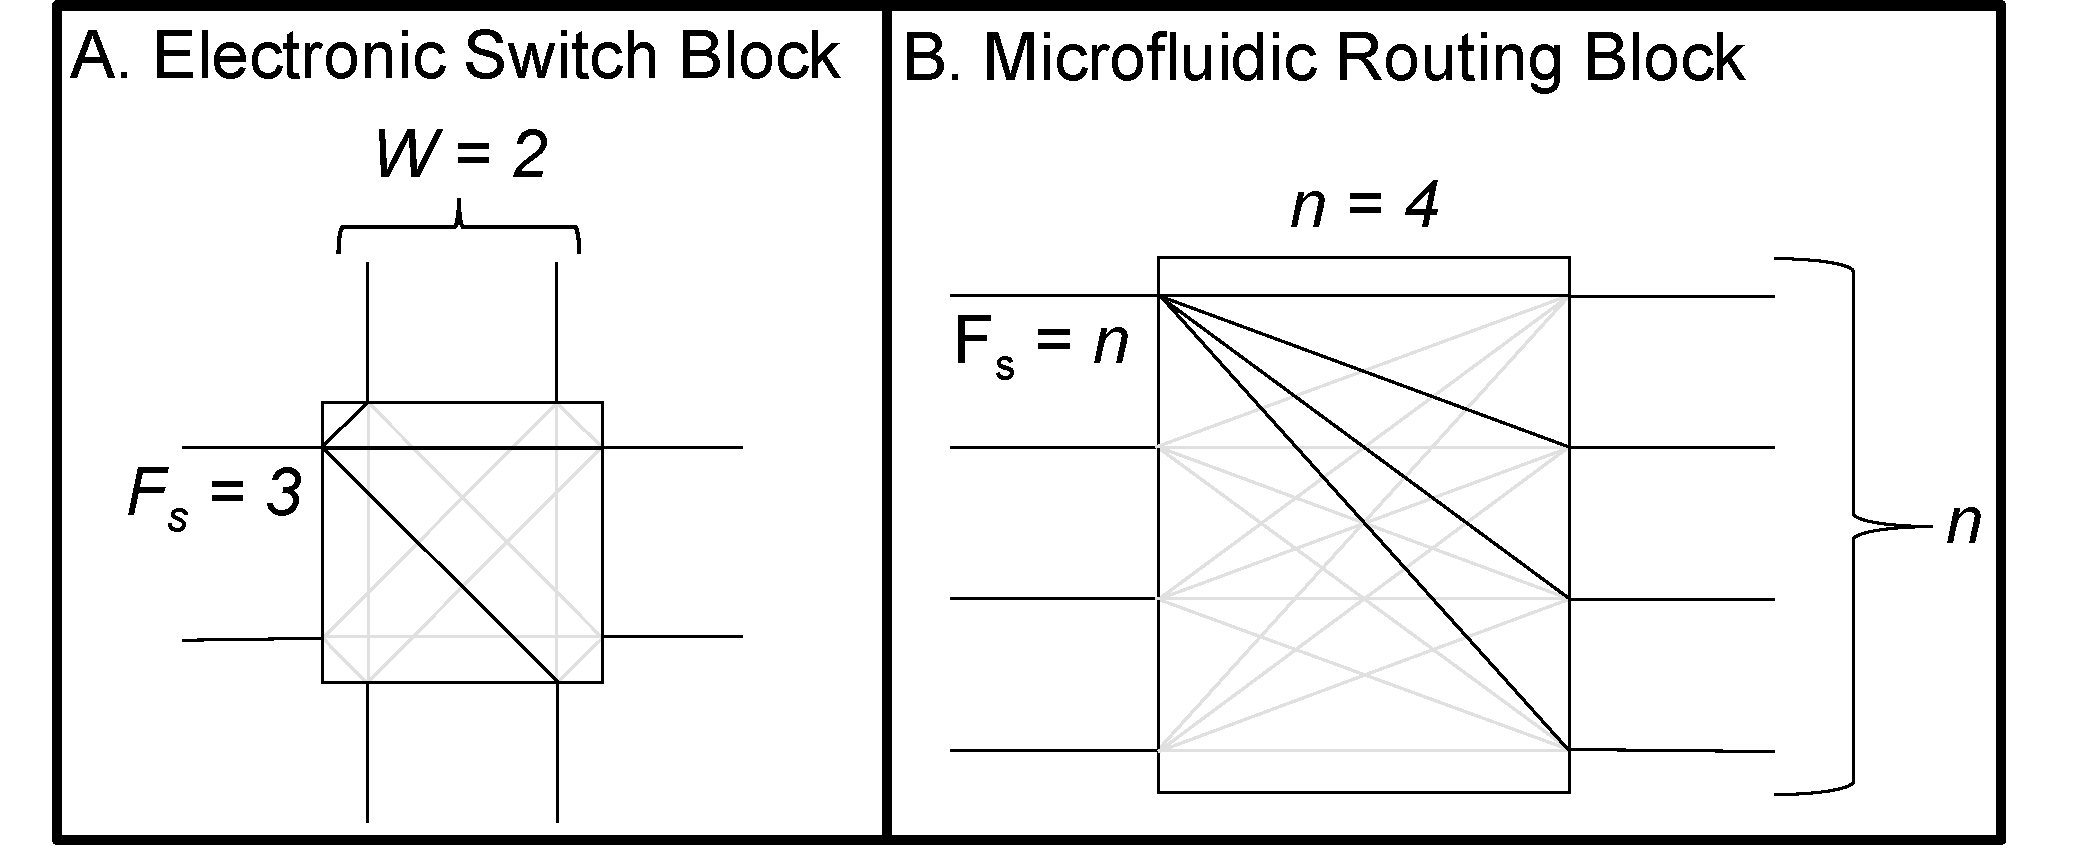
\includegraphics[width=15cm]{fig8.pdf}
      \medskip
     \end{minipage}\hfill
     \caption[Electronic and Microfluidic programmable routing blocks]{Electronic (A.) and Microfluidic (B.) programmable routing blocks. The channel width ($W$) and flexibility ($F_s$) of the electronic switching block (A.) is two and three, respectively. These switching block attributes are the same as the ones used in Figure \ref{fig:fpgaArchAndRouting}A and \ref{fig:fpgaArchAndRouting}B.}
	\label{fig:switchBlocks}
\end{figure}

Programmable routing structures within an island-style FPGA can take on one of two general forms: \textbf{switching blocks} or \textbf{connection blocks}. Connection blocks are used to connect the prefabricated wire segments directly to CLBs. Switching blocks are used to connect prefabricated wire segments at dimensional intersections within the 2D or 3D array; for example, a 2D island-style FPGA architecture places a switching block at all intersections of vertical and horizontal prefabricated wire segments \cite{schmit2002fpga}, as Figure \ref{fig:fpgaArchAndRouting}A demonstrates. As shown in Figure \ref{fig:switchBlocks}, $W$ denotes the number of prefabricated wire segments on each side of the switching block, while $F_s$ denotes the switching block's flexibility, i.e., the number of possible routes for each prefabricated wire segment entering the switching block. Figure \ref{fig:fpgaArchAndRouting}B is an example of signal routing using a switching block with $W=2$ and $F_s=3$. 


A transposer-based routing fabric can be viewed as having the functionality of a combination switching block and connection block, which we will call a \textbf{routing block}, in a 1D FPGA. A microfludic routing block can be described in the same terms as an FPGA switching block. As shown in Figure \ref{fig:fpgaArchAndRouting}C, the routing block developed in this work has a flexibility $F_s=n$ and width $W=n$. Microfluidic \textbf{functional blocks} can take the form of any microfluidic primitive such as cell traps, gradient generators, or optical reporting areas. These functional blocks need not be uniform with regard to the number of input or output ports between blocks, nor must they be symmetric in the number of input and output ports in the same block, as Figure \ref{fig:fpgaArchAndRouting}C shows. Functional blocks may take on any class of microfluidic function including, but not limited to, combining operations (mixing, droplet generation, etc.), biological operations (cell culture, polymerase chain reaction (PCR), etc.), or measurement/sensing operations (microscopy, pH, etc.). 

In microfluidic and electronic FPGA architectures, elementary functions are performed in functional blocks and CLBs, respectively. More complex operations are accomplished by chaining multiple blocks together using our routing fabric. Since all elements are modular and programmable, both architectures provide flexibility that is impossible to achieve in traditional, application-specific chips.  Chaining multiple primitives through microfluidic routing blocks has compounding effects on a chip's flexibility and functional capability in a manner similar to that of an FPGA. This concept is described in further detail in Section \ref{sec:example}. These novel capabilities are impossible in a continuous-flow microfluidic device without the capability of dynamic fluid routing provided by the transposer routing fabric.


\begin{figure}[h]
  \begin{minipage}[t]{0.99\linewidth}\centering
    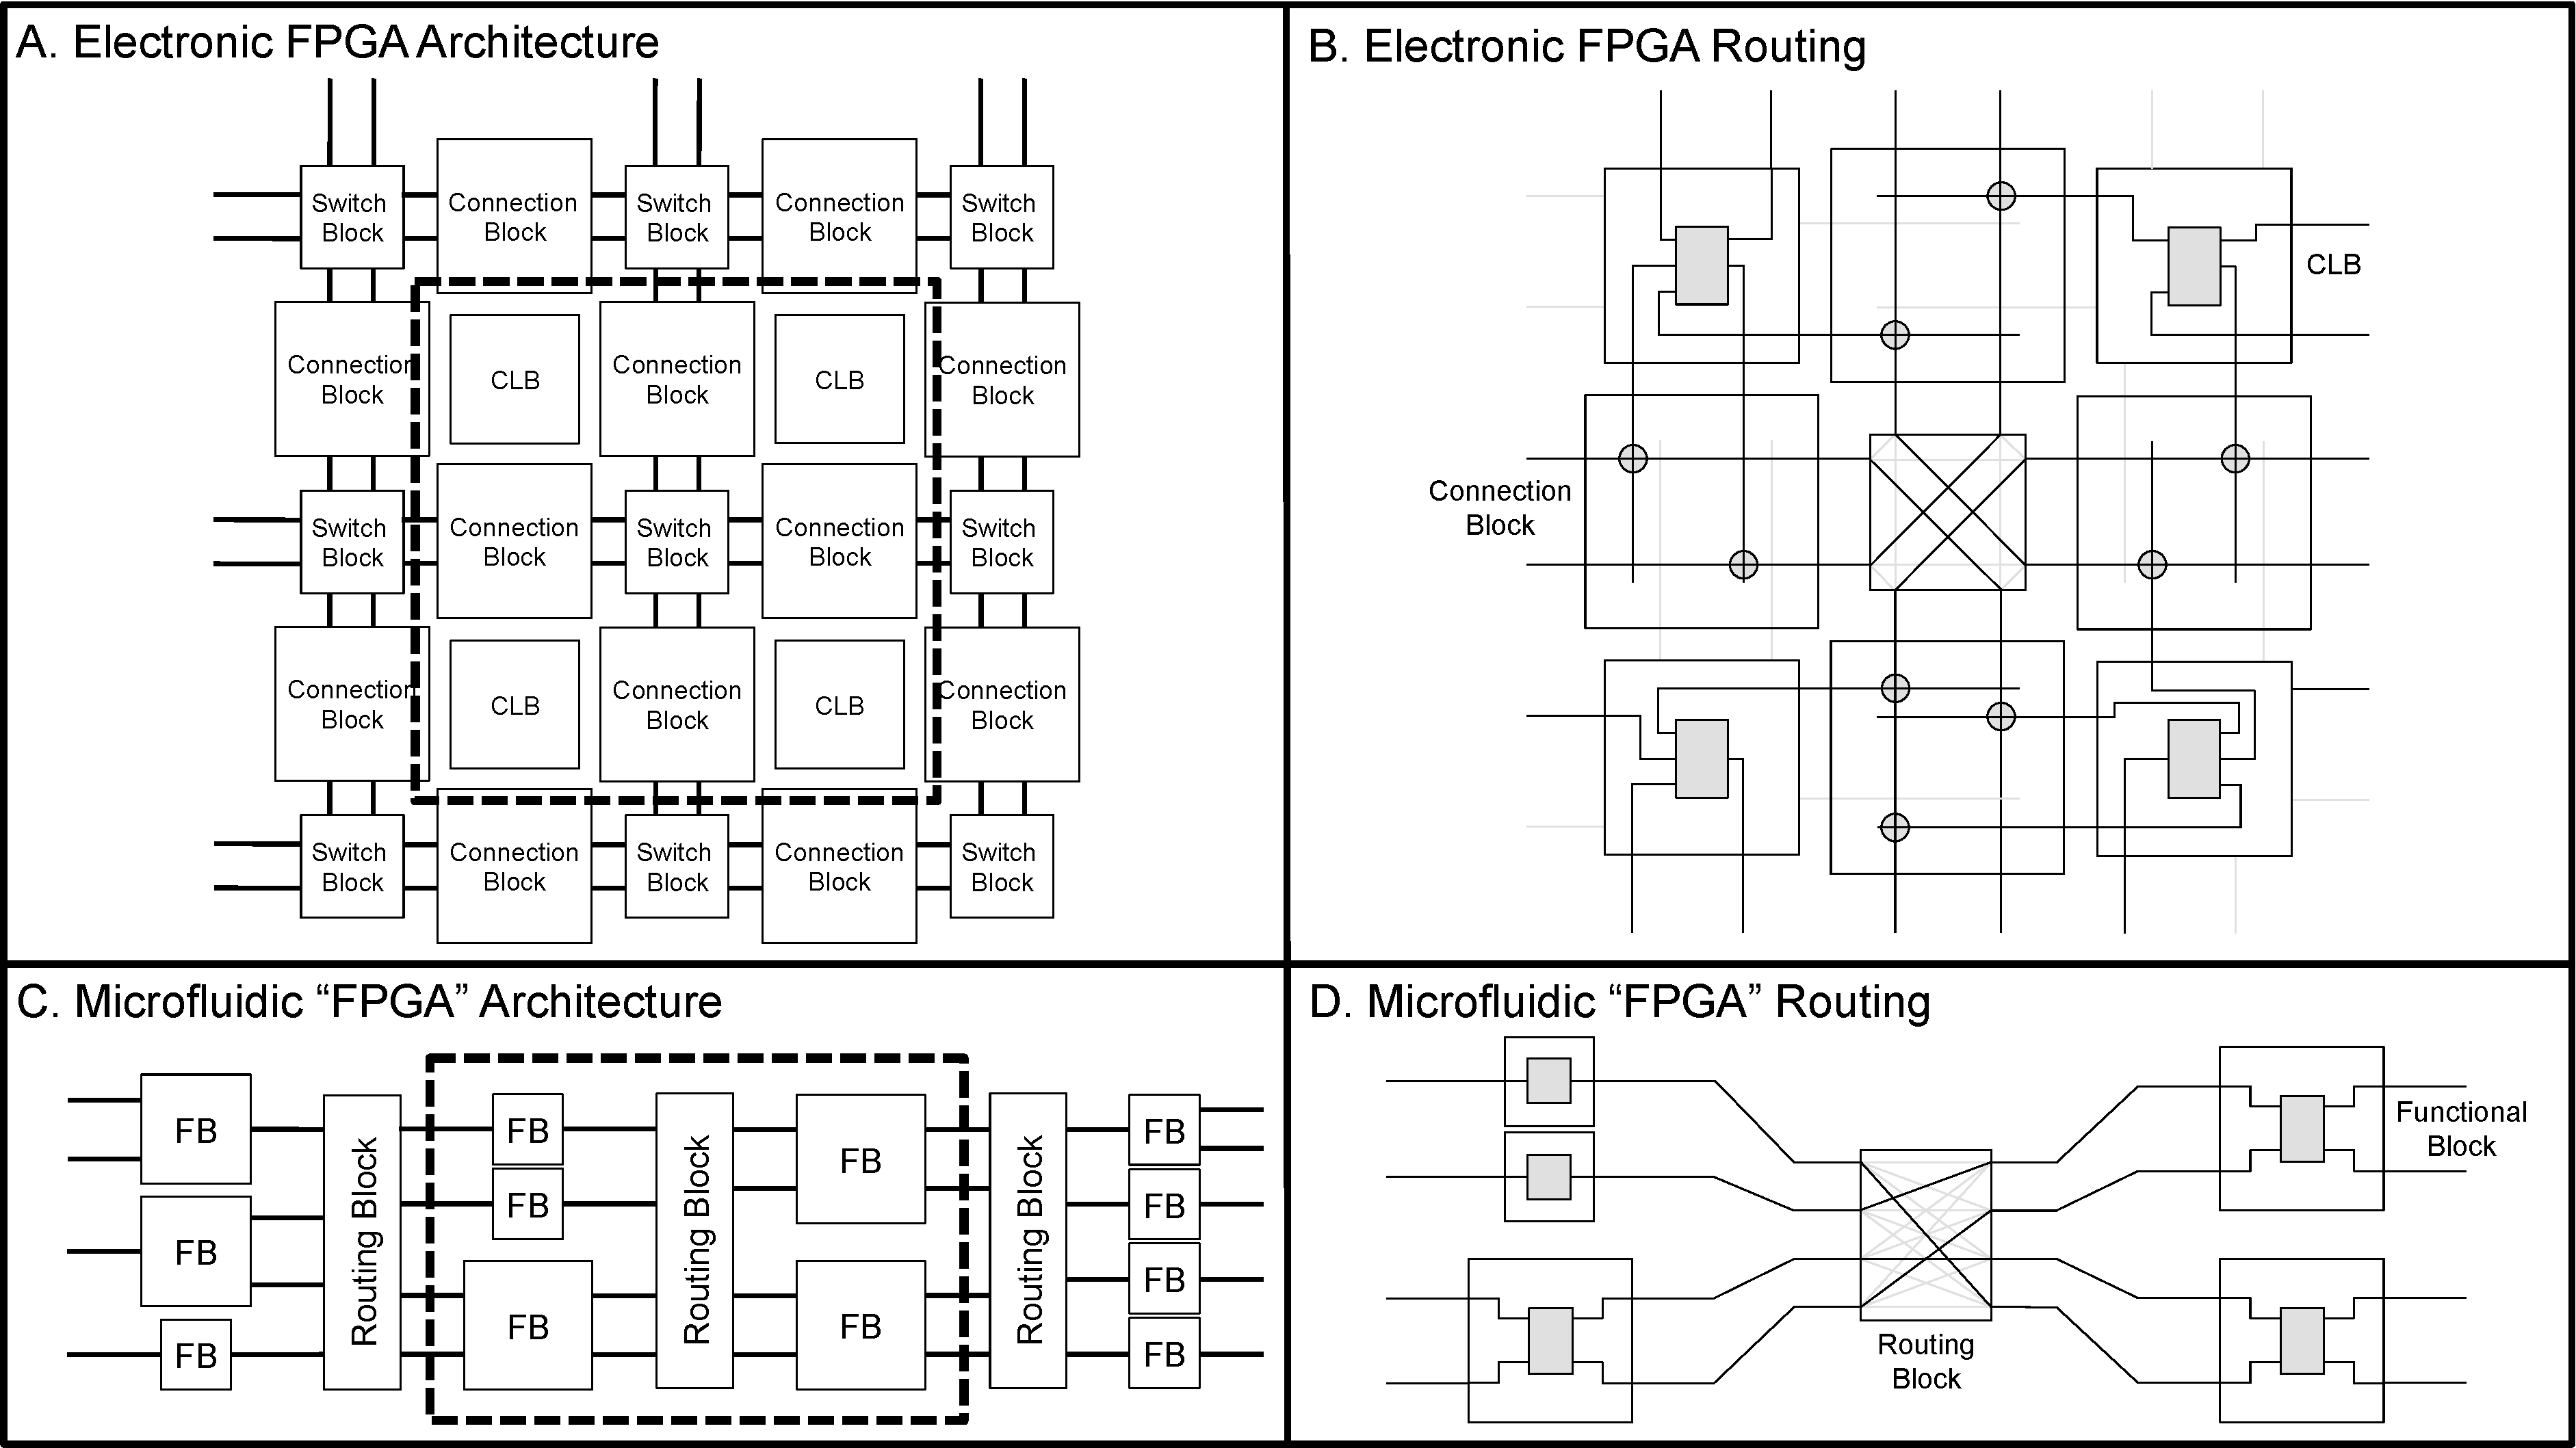
\includegraphics[width=15cm]{fig9.pdf}
    \medskip
  \end{minipage}\hfill
  \caption[Electronic and Microfludic programmable architectures]{Electronic and Microfluidic programmable architectures. A 2D, island-style Electronic FPGA architecture (A.) with example routing (B.) of the area of interest indicated by a dashed line in A. A transposer-based microfluidic chip architecture (C.) with example routing of area of interest (D.) indicated by a dashed line in C. Microfluidic functional blocks (FB) can be any continuous-flow microfluidic function such as mix, measure, etc. The microfluidic architecture in C. demonstrates that functional blocks need not be uniform (i.e., all have the same number of input/output channels). Grey lines in B. and D. indicate unconnected paths.}
	\label{fig:fpgaArchAndRouting}
\end{figure}

\subsection{Example Architecture}
\label{sec:example}
Consider a lab that utilizes two distinct microfluidic devices. The first device is a two-stage microfluidic designed to mix a particle stream with a buffer stream and then perform separation as part of a protocol for rare cell isolation \cite{pamme2007continuous}. The second device is also a two-stage microfluidic but instead of performing mixing and separation, this device utilizes cell trapping followed by a thermal treatment within a temperature-controlled reaction chamber as part of a polymerase chain reaction (PCR) protocol \cite{zhang2006pcr}. If these two distinct chips are brought together, with a single transposer separating the two stages, a flexible architecture is created with novel functionality. For example, the two independent chips were originally only capable of mixing followed by separation and trapping followed by temperature cycling, respectively; the new chip, incorporating a single transposer, is now capable of mixing followed by temperature cycling, which could be useful in chemical synthesis \cite{jensen2014tools}, and at the same time is capable of trapping followed by separation, which is part of a protocol for debulking platelets from blood samples \cite{shields2015microfluidic}.

	Figure \ref{fig:example} shows a schematic representation of all possible functionalities derived from such an architecture. The addition of more functional blocks vertically (i.e., increasing $n$ on a routing block) increases the number of possible simultaneous operations the chip can perform, while adding more functional blocks horizontally, with each stage separated by a routing block, increases the number of possible sequential operations. This specificity achieved through well-tested and characterized functional blocks (ex., mixers, separators, cell traps and reaction chambers) coupled with the flexibility of a programmable routing architecture unlocks a new category of programmable devices made possible only through arbitrary, continuous-flow microfluidic routing. 


Functional blocks may have incompatible channel geometries relative to other functional blocks in a larger architecture. This issue can be mitigated by modifying the primitive's channel geometries for each differing channel of interest. This would only be necessary should a channel reduction or expansion impede function and if the differing channels require rerouting; otherwise, these geometries would be considered internal to a functional block and not part of the routing fabric. Should a chip architecture require rerouting of multiple channels of differing dimensions, this would result in separate routing fabrics for each channel geometry that requires rerouting. The routing fabric is flexible such that a device containing separate routing fabrics, based on channel dimensions, could be integrated without any modifications to the algorithmic framework.

\begin{figure}[h]
     \begin{minipage}[t]{0.99\linewidth}\centering
      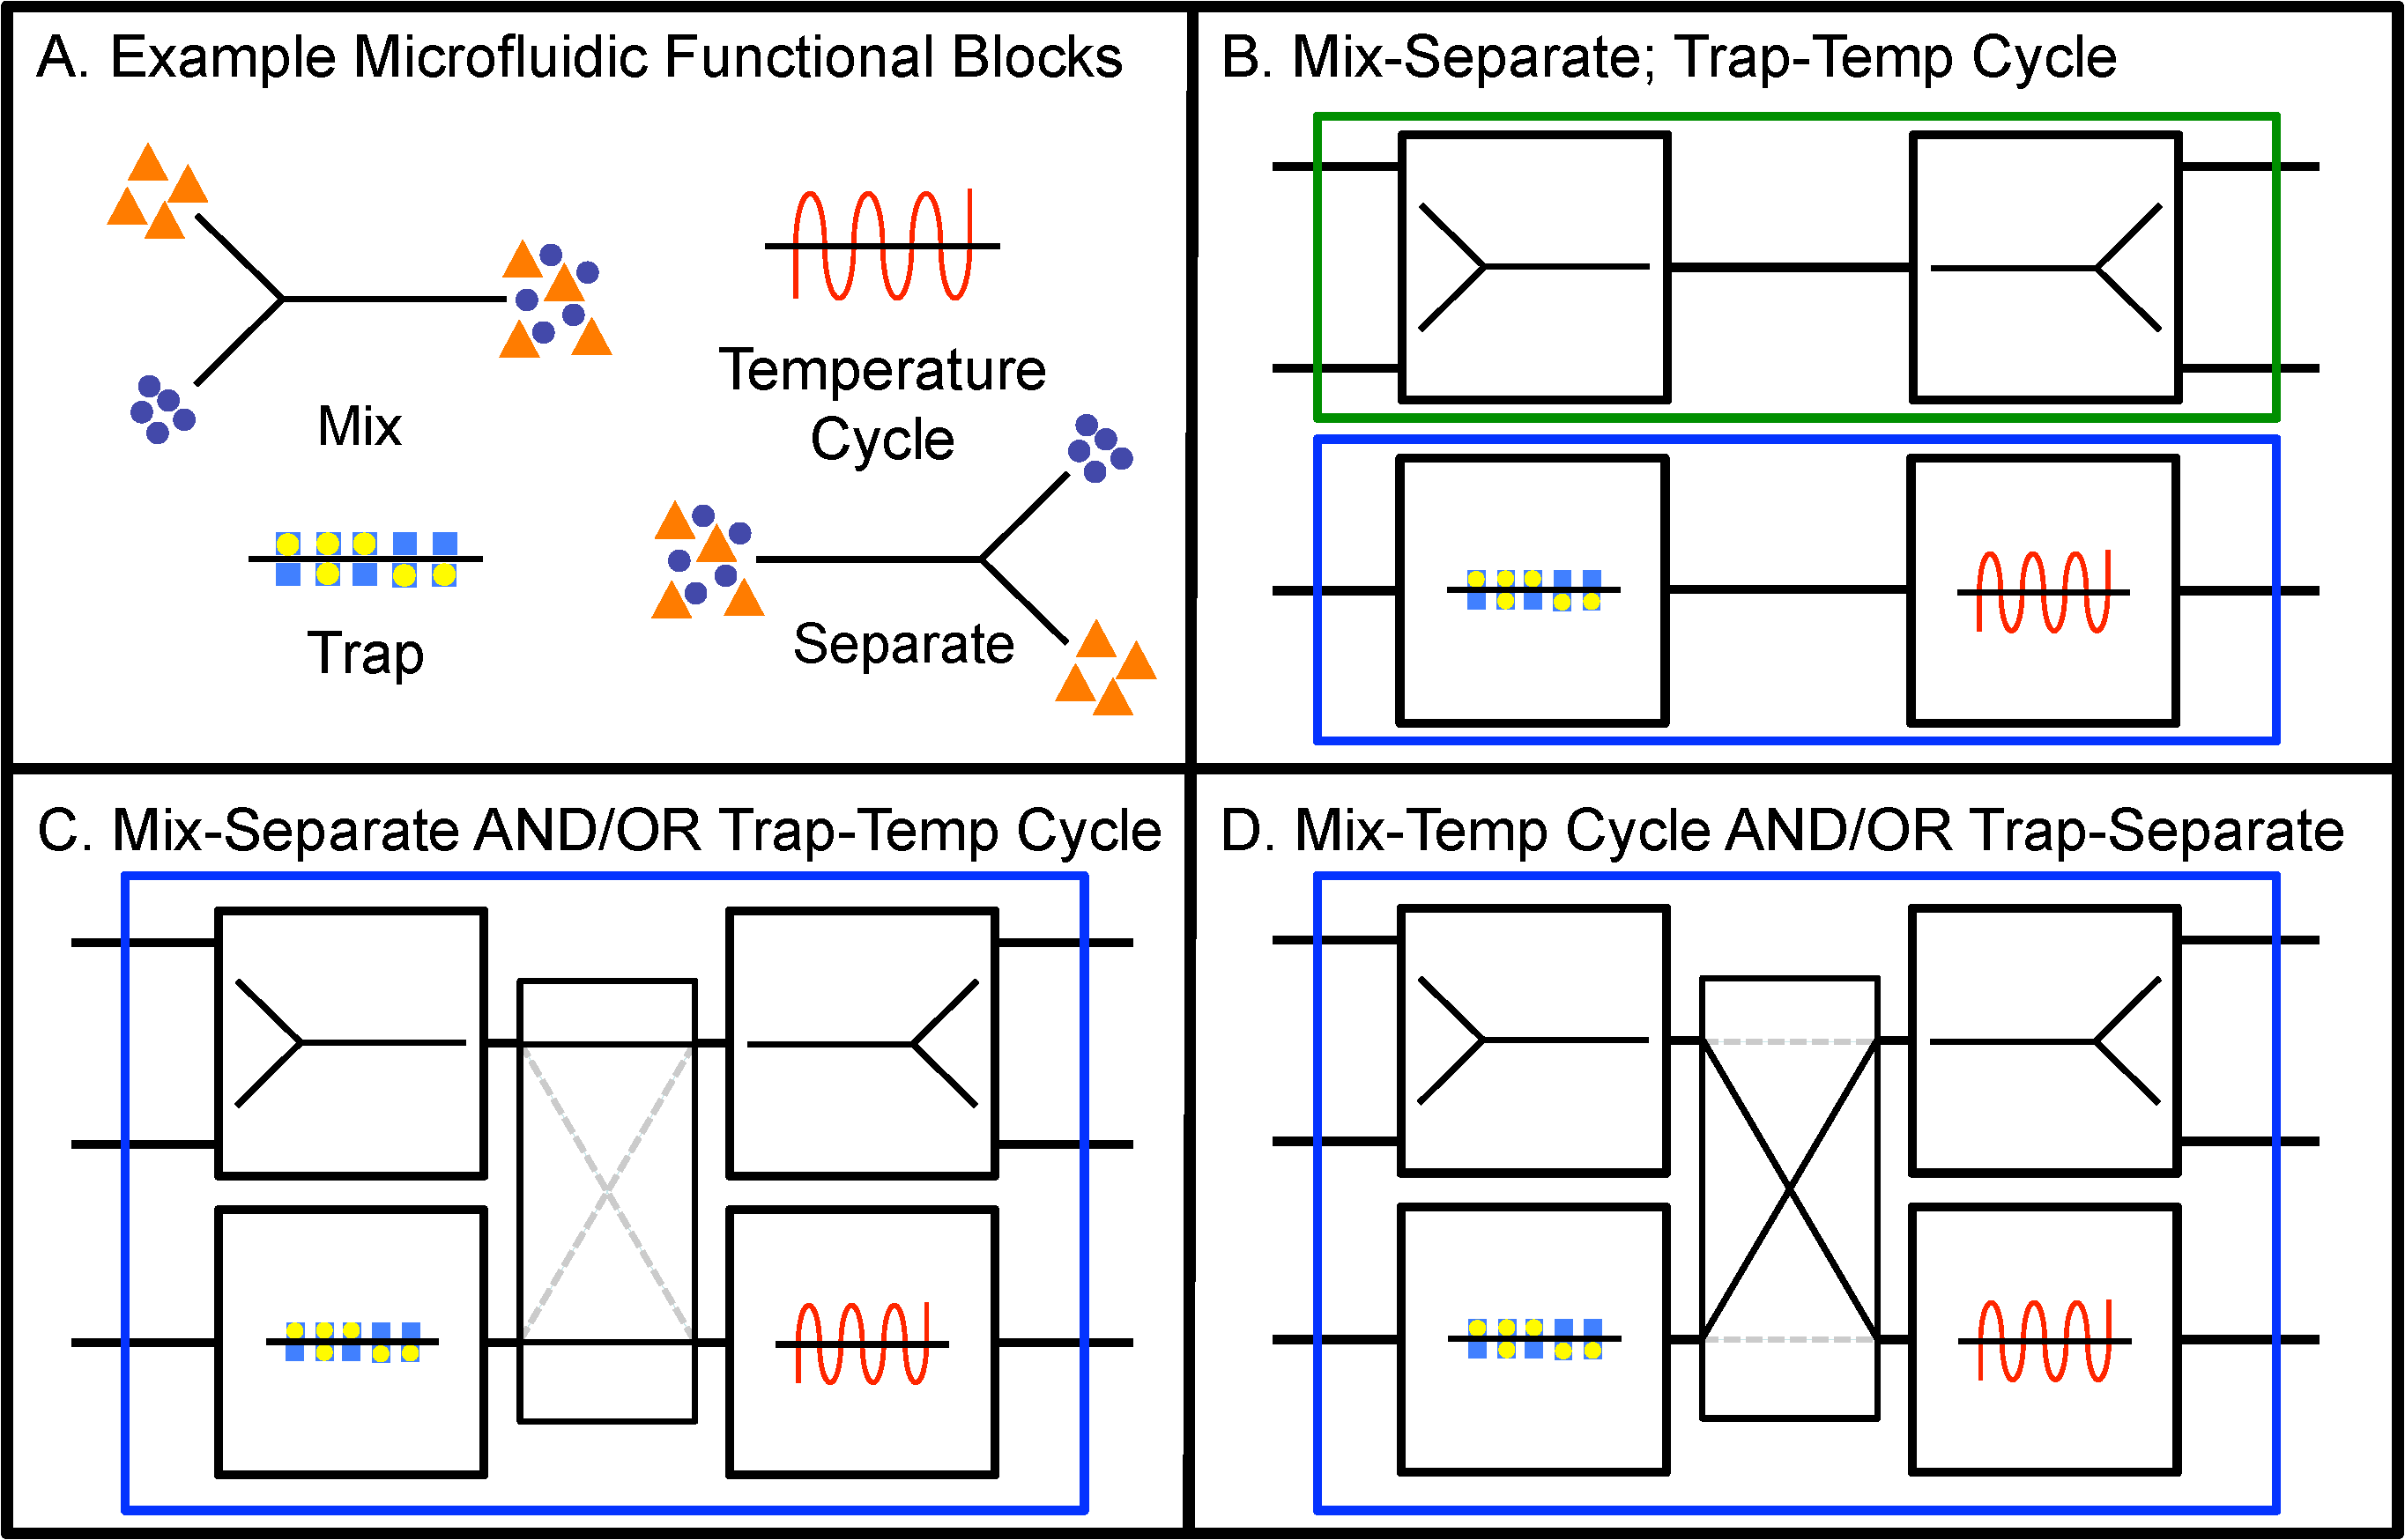
\includegraphics[width=14cm]{fig10.pdf}
      \medskip
     \end{minipage}\hfill
     \caption[Example of a functional, programmable microfluidic architecture]{Example architecture utilizing a single transposer. Microfluidic functional blocks (A.) are connected via static channels to form two separate devices (B.) the functions of which are immutable. One device can perform mixing and then separation, while the other can perform cell trapping and then temperature cycling. A transposer is used to join the functional blocks in lieu of static channels (C. and D.). This results in two novel functions, mix then temperature cycle and trap then separate (D.). Additionally, The single microfluidic chip is able to perform both functions shown in C. simultaneously as well as both functions in D.}
	\label{fig:example}
\end{figure}

\subsection{Dynamic Reconfiguration}
Integrating intermediate sensing operations as functional blocks within a transposer-based microfluidic routing architecture unlocks a unique ability to dynamically reroute fluids based on real-time measurements. This is particularly valuable in experiments involving fluidic operations that depend on dynamic fluidic variables such as directed evolution \cite{wang2014microfluidic}, refinement \cite{swain2013thinking} and genetic logic \cite{tamsir2011}. However, reconfiguration of the routing fabric during run time carries a distinct limitation whereby at the moment of reconfiguration, a contaminated plug of liquid will propagate through the device. The problem is analogous to the concept in digital electronics of a dynamic discipline \cite{Harris+Harris}. The dynamic discipline affirms that the output of a digital logic element (ex. a flip flop) is not deterministic if queried inside of its established propagation delay. Extending this analogy to microfluidic routing, it can be stated that if a transposition occurs within channels containing functionally orthogonal fluids (so as to prevent permanent contamination downstream) that the output of the system will be valid only after waiting for the contaminated plugs to propagate through the device.



\subsection{Future Work}
One particular strength of this work is the technology-agnostic manner in which the framework was built. This means that the transposer primitive can be optimized to suit any control or fabrication environment so long as the basic functionality shown in Figure \ref{fig:modes} is retained. The optimal transposer primitive may look dramatically different between experimentalists performing separation using acoustophoresis \cite{petersson2007free} versus filtration \cite{pamme2007continuous}, yet the routing framework would be identical.

Since each primitive only requires two control lines, which are of equipotential and toggled in a manner similar to the microfluidic multiplexor previously described \cite{thorsen2002}, the optimization of control lines based on variable routing constraints is a solvable problem.

Finally, the formulation of a flexible microfluidic architecture that encompasses a maximum subset of microfluidic assays is under development. This chip would allow experimentalists to fabricate devices in bulk, yet maintain maximum flexibility to perform a large range of assays and experiments using the same chip. Organic software will accompany this architecture and serve to integrate device-level microfluidic control with assay-level specification. This effectively raises the level of abstraction for the microfluidic experimentalist and frees the community from the need to design, fabricate, and control singular microfluidic architectures for each experiment; rather, the experimentalist will reprogram the same chip architecture for many types of experiments through the same control environment.

\section{Conclusions}
This work demonstrates a novel microfluidic routing fabric for continuous-flow devices using a scalable primitive called a transposer. The fabric exists independent of any optimizations made to the primitive itself. We proved that fluidic routing through the fabric is extensible and developed algorithms to do so. We then integrated the fabric into a larger architecture towards the development of a programmable continuous-flow microfluidic device akin to the class of electronic devices known as FPGAs. 

The barrier to entry for continuous-flow microfluidics can be prohibitively high, yet the benefits of microfluidic technology are too good to ignore \cite{whitesides2006}. This work serves to introduce a new class of programmable microfluidic devices aimed at decreasing the design, fabrication, and operational costs of continuous-flow microfluidics thus increasing the accessibility of microfluidic technology. It is our hope that programmable continuous-flow microfluidics could serve as the catalyst towards microfluidic ubiquity as programmable electronics was for electronic computing.
